\documentclass[noinstructornotes]{ximera}
%handout:  for handout version with no solutions or instructor notes
%handout,instructornotes:  for instructor version with just problems and notes, no solutions
%noinstructornotes:  shows only problem and solutions

%% handout
%% space
%% newpage
%% numbers
%% nooutcomes

%I added the commands here so that I would't have to keep looking them up
%\newcommand{\RR}{\mathbb R}
%\renewcommand{\d}{\,d}
%\newcommand{\dd}[2][]{\frac{d #1}{d #2}}
%\renewcommand{\l}{\ell}
%\newcommand{\ddx}{\frac{d}{dx}}
%\everymath{\displaystyle}
%\newcommand{\dfn}{\textbf}
%\newcommand{\eval}[1]{\bigg[ #1 \bigg]}

%\begin{image}
%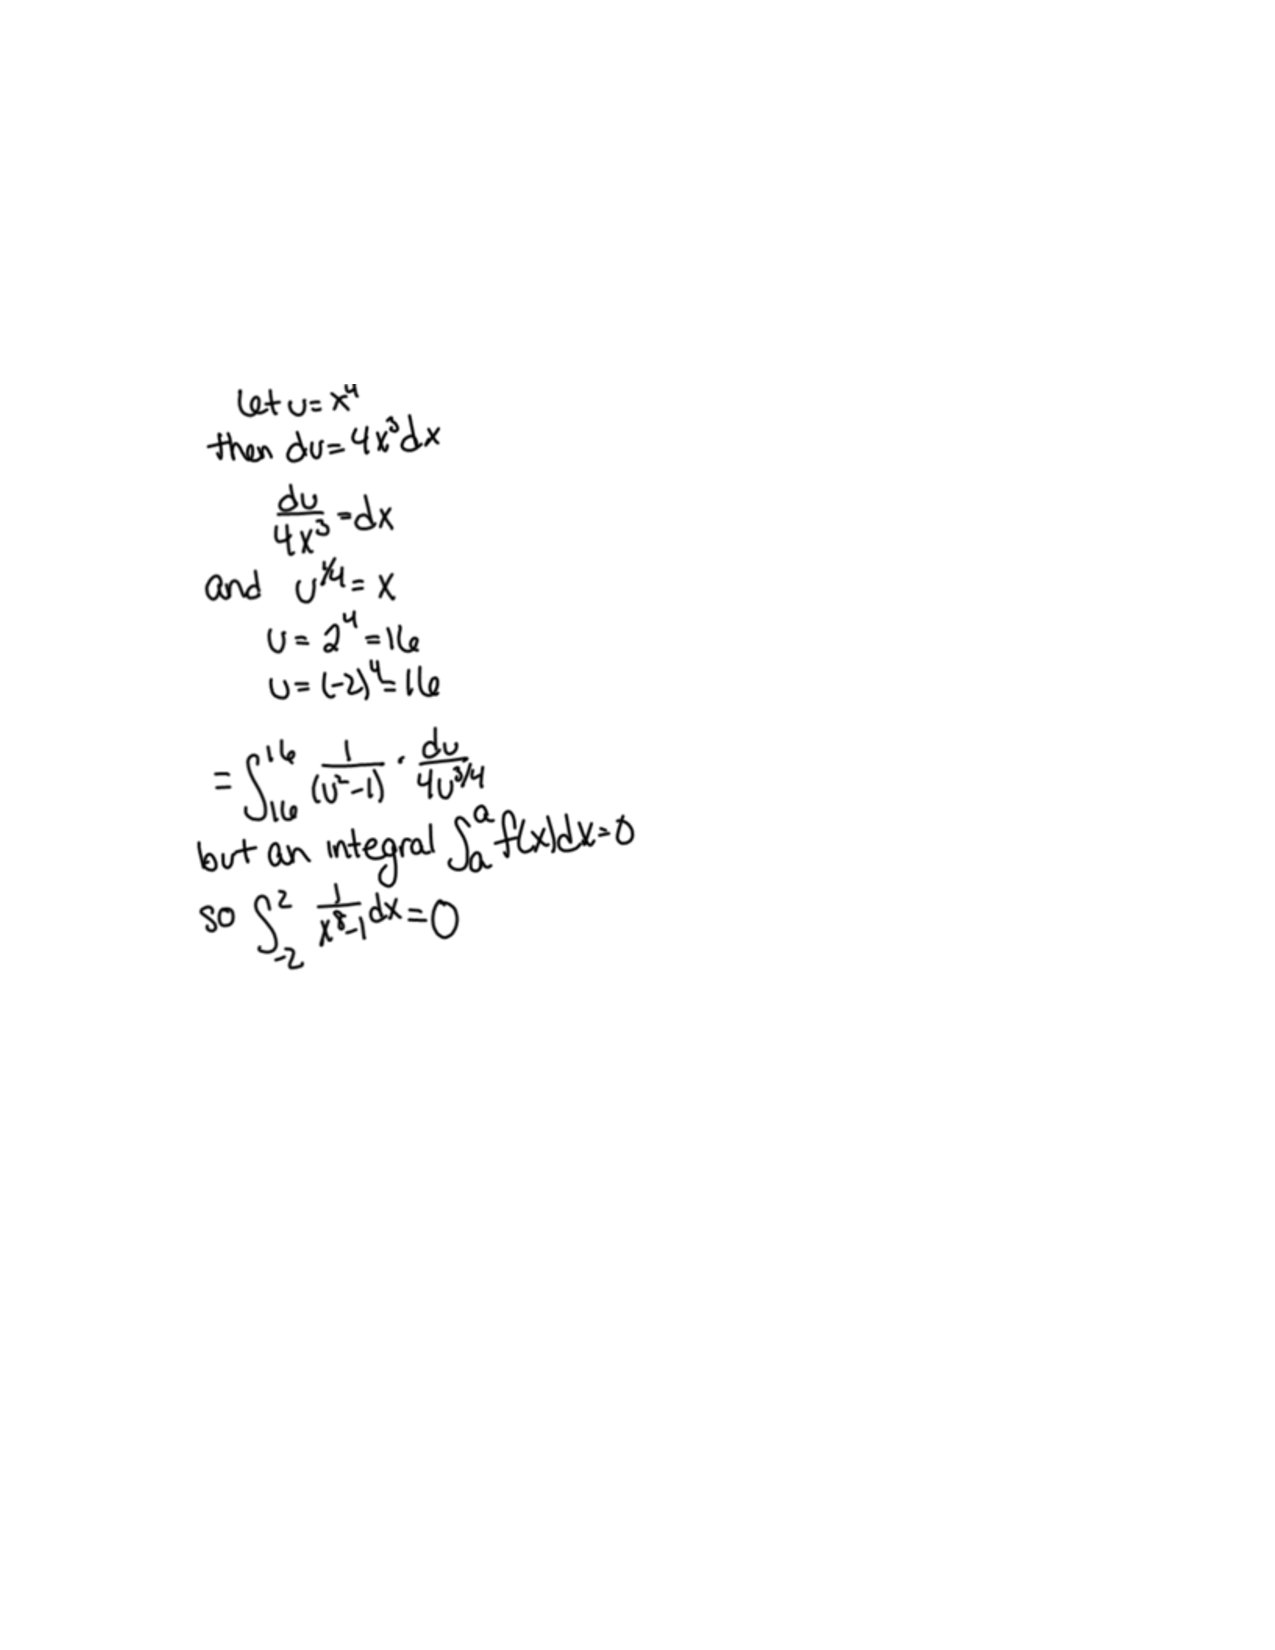
\includegraphics[trim= 170 420 250 180]{Figure1.pdf}
%\end{image}

%add a ``.'' below when used in a specific directory.
\newcommand{\RR}{\mathbb R}
\renewcommand{\d}{\,d}
\newcommand{\dd}[2][]{\frac{d #1}{d #2}}
\renewcommand{\l}{\ell}
\newcommand{\ddx}{\frac{d}{dx}}
\newcommand{\dfn}{\textbf}
\newcommand{\eval}[1]{\bigg[ #1 \bigg]}

\usepackage{multicol}

\renewenvironment{freeResponse}{
\ifhandout\setbox0\vbox\bgroup\else
\begin{trivlist}\item[\hskip \labelsep\bfseries Solution:\hspace{2ex}]
\fi}
{\ifhandout\egroup\else
\end{trivlist}
\fi} %% we can turn off input when making a master document

\title{Section 11.2: Polar coordinates}  

\begin{document}
\begin{abstract}		\end{abstract}
\maketitle












\section{Group work:}








%problem 1
\begin{problem}
Plot the following (polar) points in the $xy$-plane and then rewrite them as rectangular coordinates.
	\begin{multicols}{4}
	\begin{enumerate}
	\item  $\left( 3, \frac{5 \pi}{4}   \right) $
	\item  $\left( 3, - \frac{5 \pi}{4}   \right) $
	\item  $\left( -3, \frac{5 \pi}{4}   \right) $
	\item  $\left( -3, - \frac{5 \pi}{4}   \right) $
	\end{enumerate}
	\end{multicols}
	
	\begin{freeResponse}
	\begin{enumerate}
	\item  
		\[
		x = 3 \cos \left( \frac{5 \pi}{4} \right) = - \frac{3 \sqrt{2}}{2}
		\]
		\[
		y = 3 \sin \left( \frac{5 \pi}{4} \right) = - \frac{3 \sqrt{2}}{2}
		\]
		
		\begin{image}
		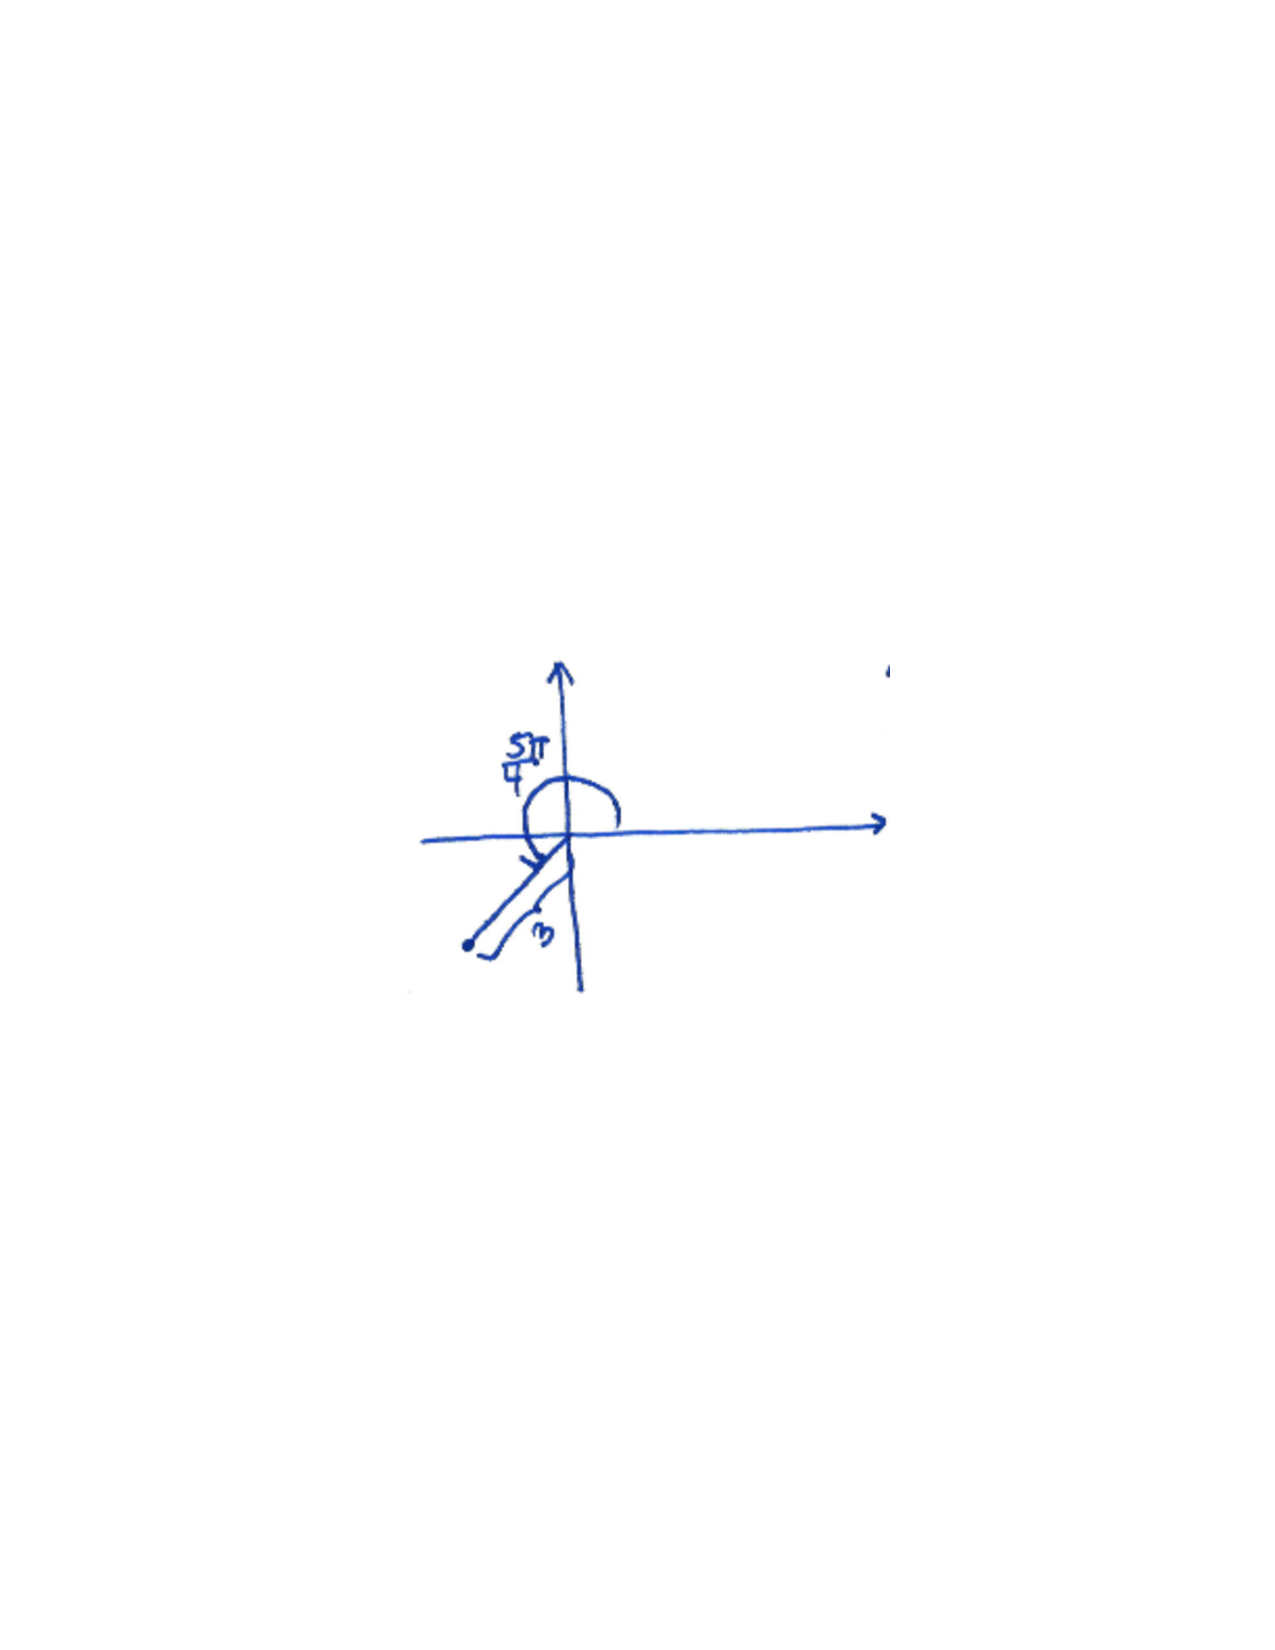
\includegraphics[trim= 170 320 170 320, scale=0.7]{Figure11-2-2.pdf}
		\end{image}
	
	\item  
		\[
		x = 3 \cos \left( - \frac{5 \pi}{4} \right) = - \frac{3 \sqrt{2}}{2}
		\]
		\[
		y = 3 \sin \left( - \frac{5 \pi}{4} \right) = \frac{3 \sqrt{2}}{2}
		\]
		
		\begin{image}
		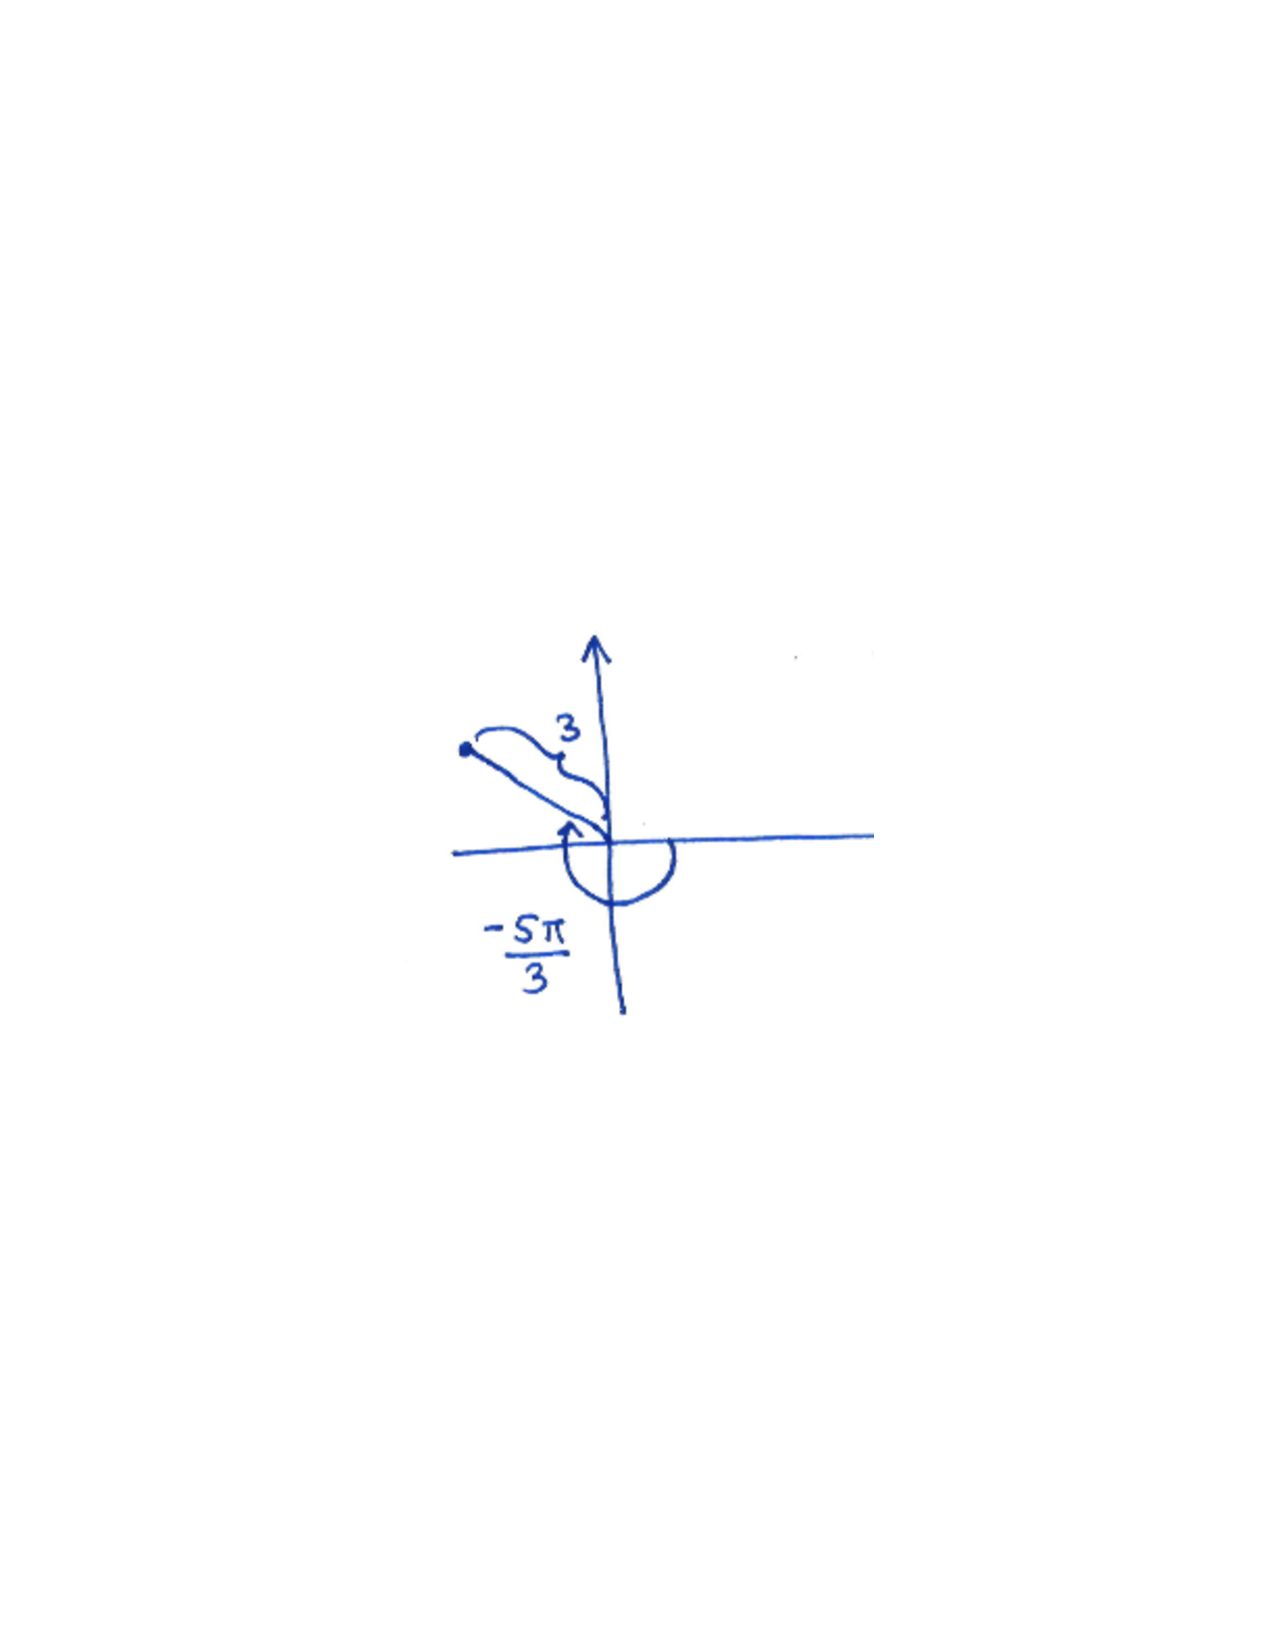
\includegraphics[trim= 170 320 170 320, scale=0.7]{Figure11-2-3.pdf}
		\end{image}
	
	\item  
		\[
		x = -3 \cos \left( \frac{5 \pi}{4} \right) = \frac{3 \sqrt{2}}{2}
		\]
		\[
		y = -3 \sin \left( \frac{5 \pi}{4} \right) = \frac{3 \sqrt{2}}{2}
		\]
		
		\begin{image}
		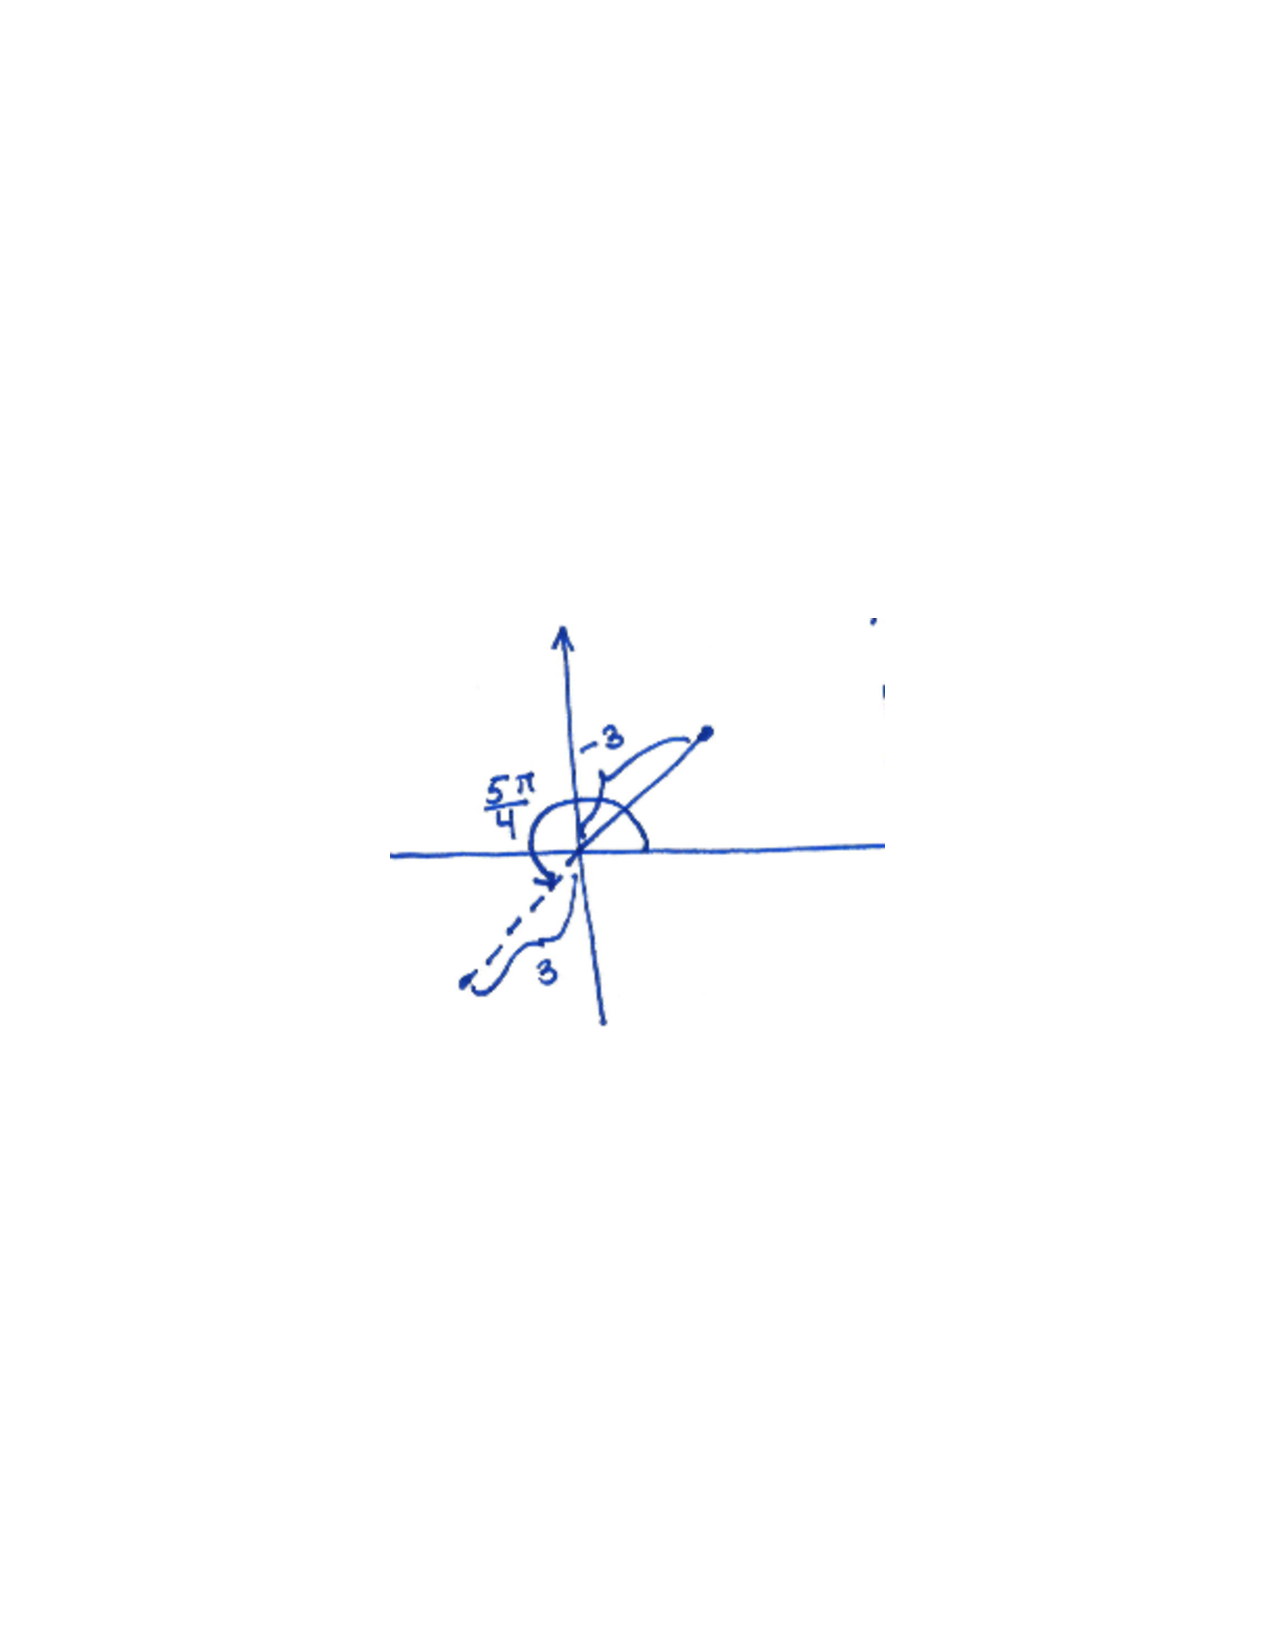
\includegraphics[trim= 170 310 170 310, scale=0.7]{Figure11-2-4.pdf}
		\end{image}
	
	\item  
		\[
		x = -3 \cos \left( - \frac{5 \pi}{4} \right) = \frac{3 \sqrt{2}}{2}
		\]
		\[
		y = -3 \sin \left( -\frac{5 \pi}{4} \right) = - \frac{3 \sqrt{2}}{2}
		\]
		
		\begin{image}
		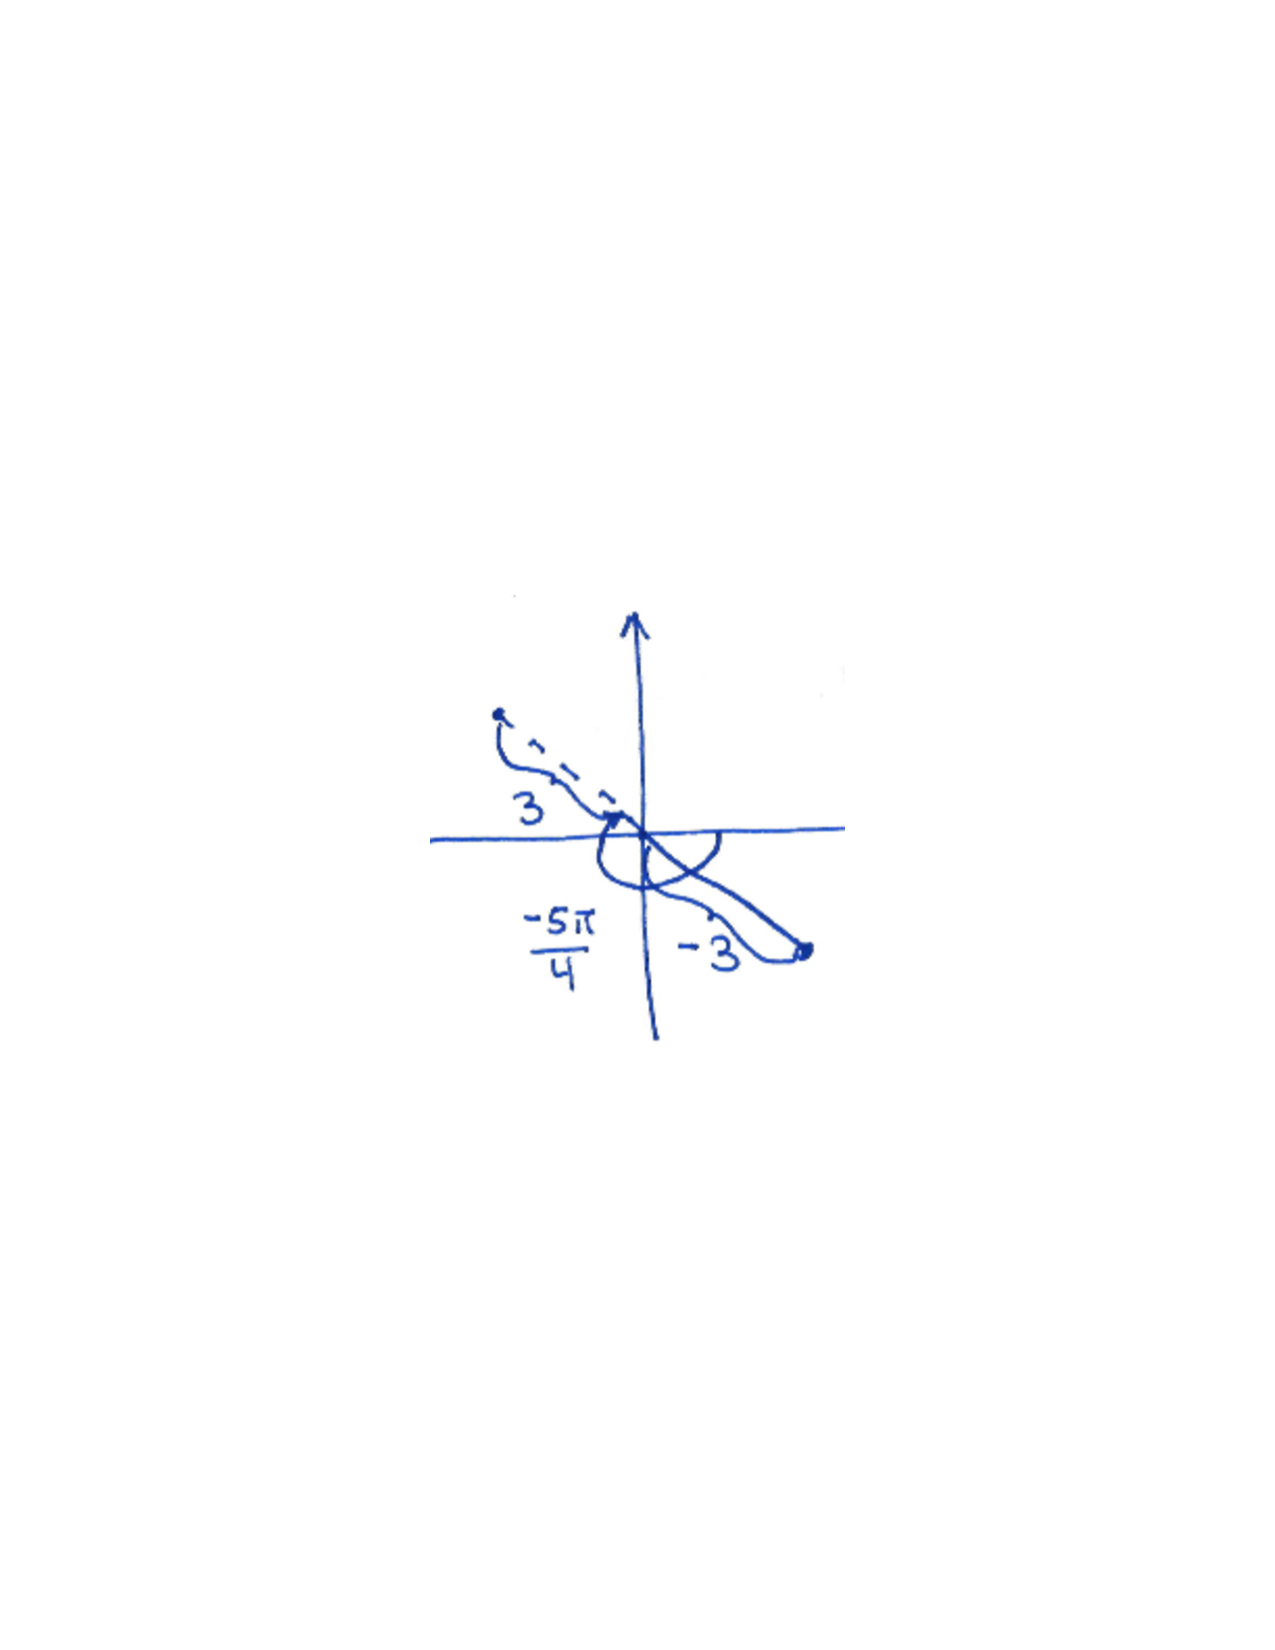
\includegraphics[trim= 170 310 170 300, scale=0.7]{Figure11-2-5.pdf}
		\end{image}
	
	\end{enumerate}
	\end{freeResponse}
	
\end{problem}

\begin{instructorNotes}
Some students will be familiar with polar coordinates while others will have never worked with them before.  
So it is very important to establish how these coordinates are measured.

Students sometimes have a difficult time dealing with negative values for $r$ as well as with working with these while graphing.  
Both this and the next problem force the students to deal with these issues.  
\end{instructorNotes}







%problem 2
\begin{problem}
Rewrite the rectangular point $(3,5)$ in polar coordinates in three different ways.
	\begin{freeResponse}
	\begin{enumerate}
	\item[i.]
		\[
		r = \sqrt{3^2 + 5^2} = \sqrt{34}	\qquad	\theta = \arctan \left( \frac{5}{3} \right)
		\]
		
		\begin{image}
		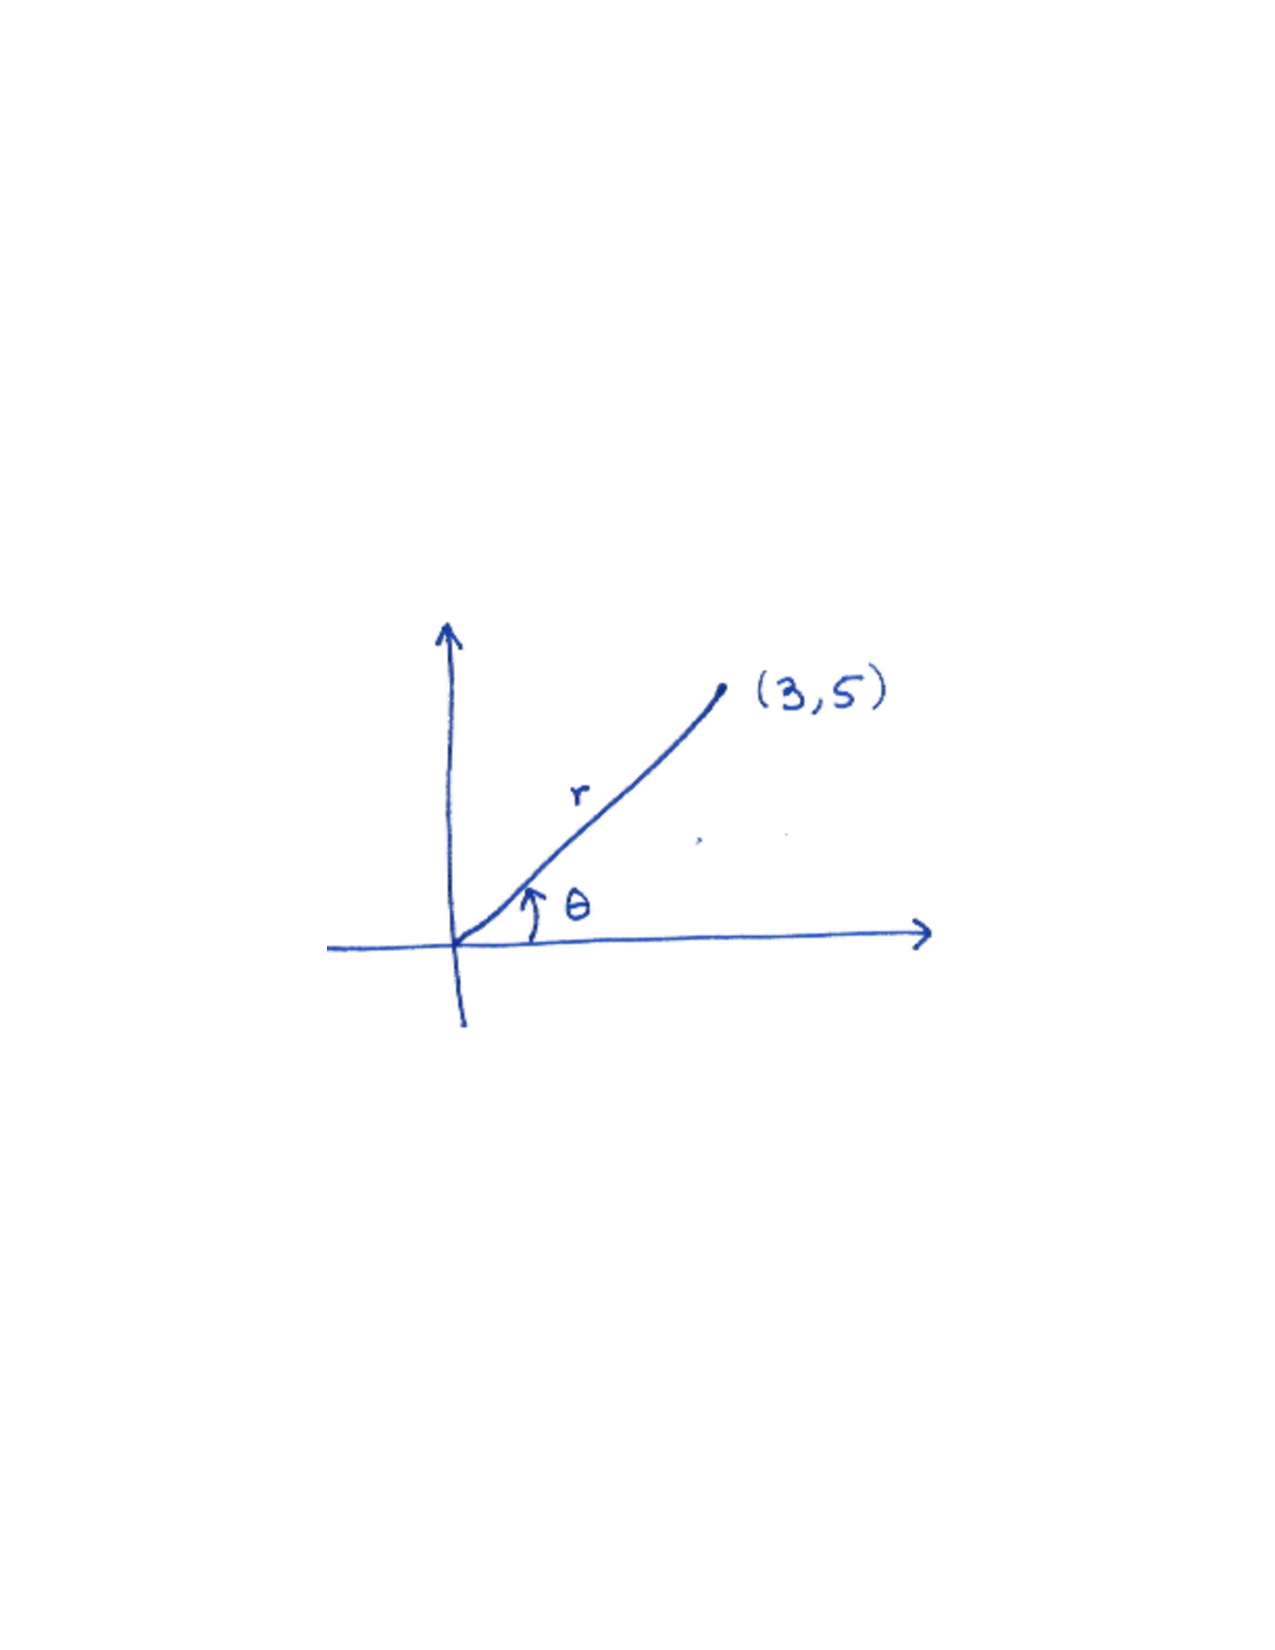
\includegraphics[trim= 170 310 170 300, scale=0.6]{Figure11-2-6.pdf}
		\end{image}
	
	\item[ii.]
		\[
		r = \sqrt{34} 	\qquad	\theta = \arctan \left( \frac{5}{3} \right) - 2 \pi
		\]
		
		\begin{image}
		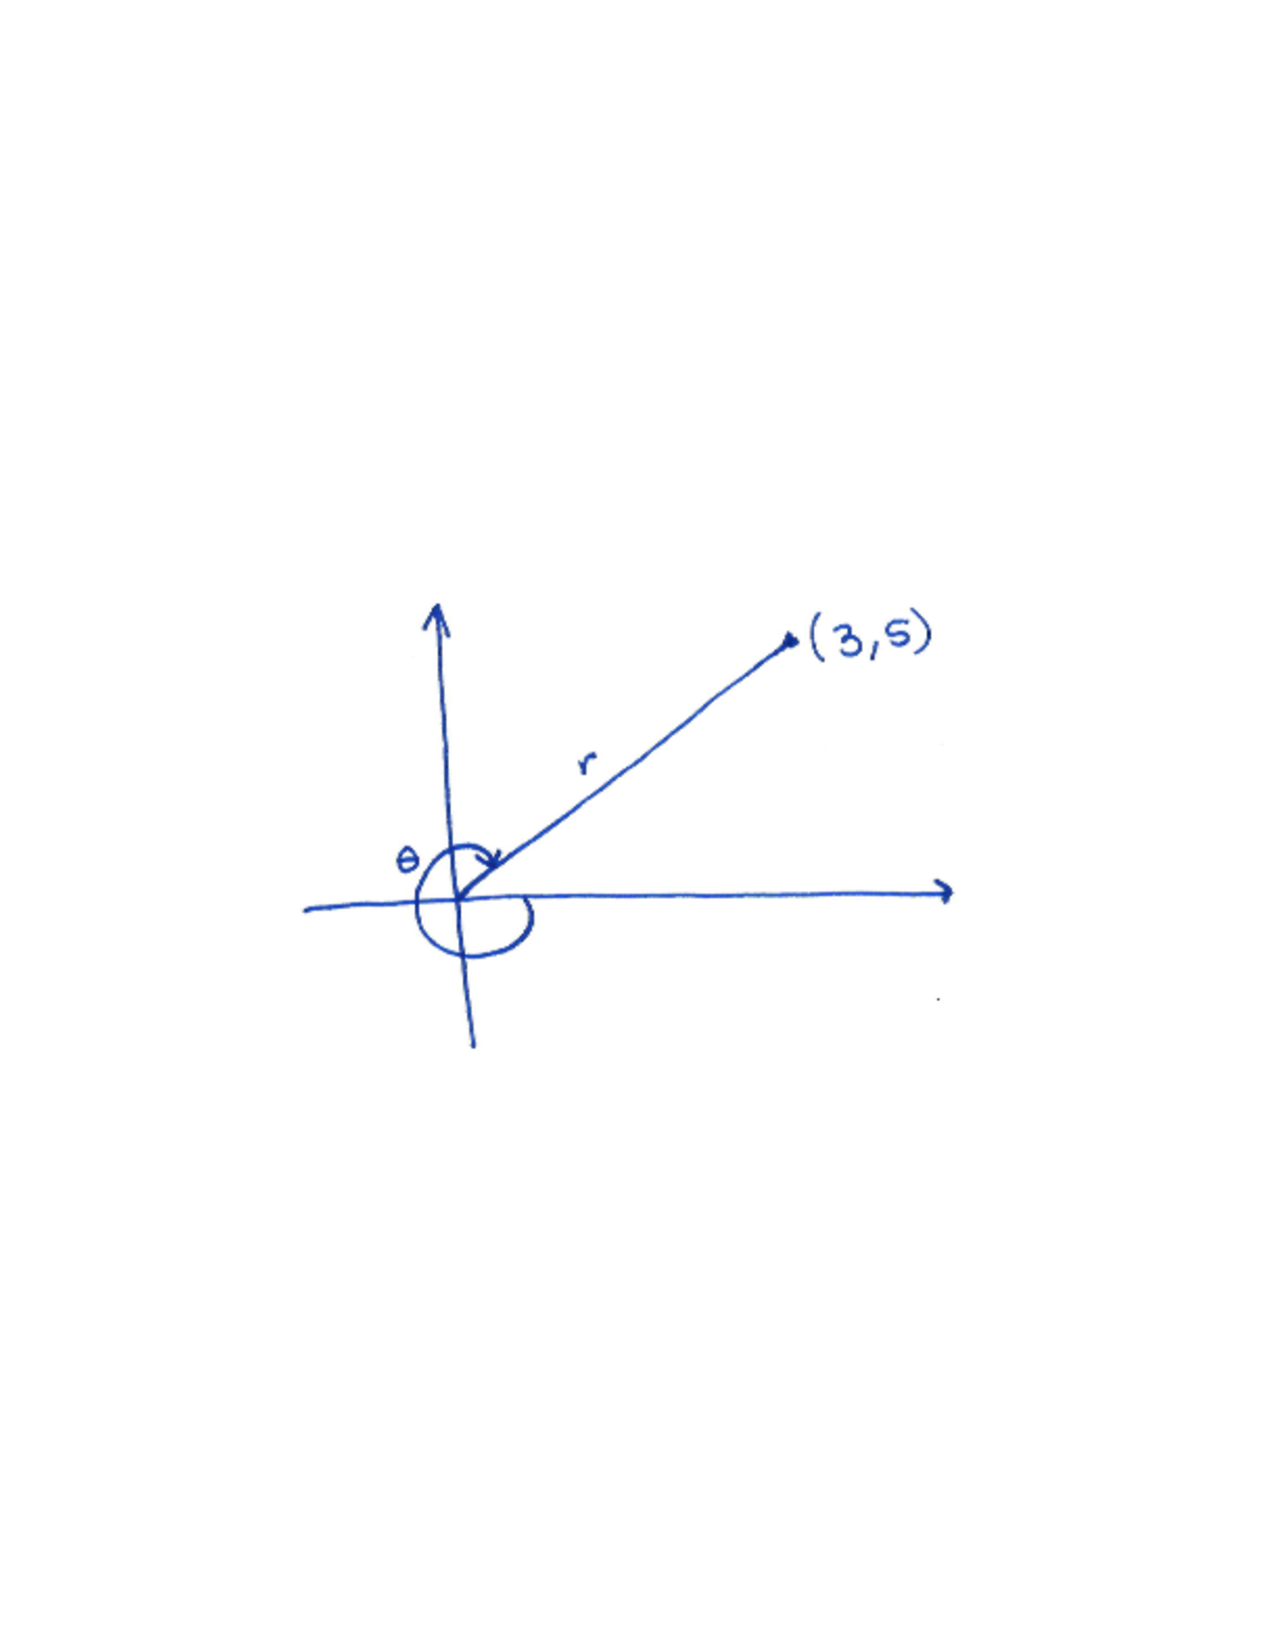
\includegraphics[trim= 170 310 170 290, scale=0.6]{Figure11-2-7.pdf}
		\end{image}
	
	\item[iii.]
		\[
		r = - \sqrt{34}	\qquad	\theta = \arctan \left( \frac{5}{3} \right) + \pi
		\]
		
		\begin{image}
		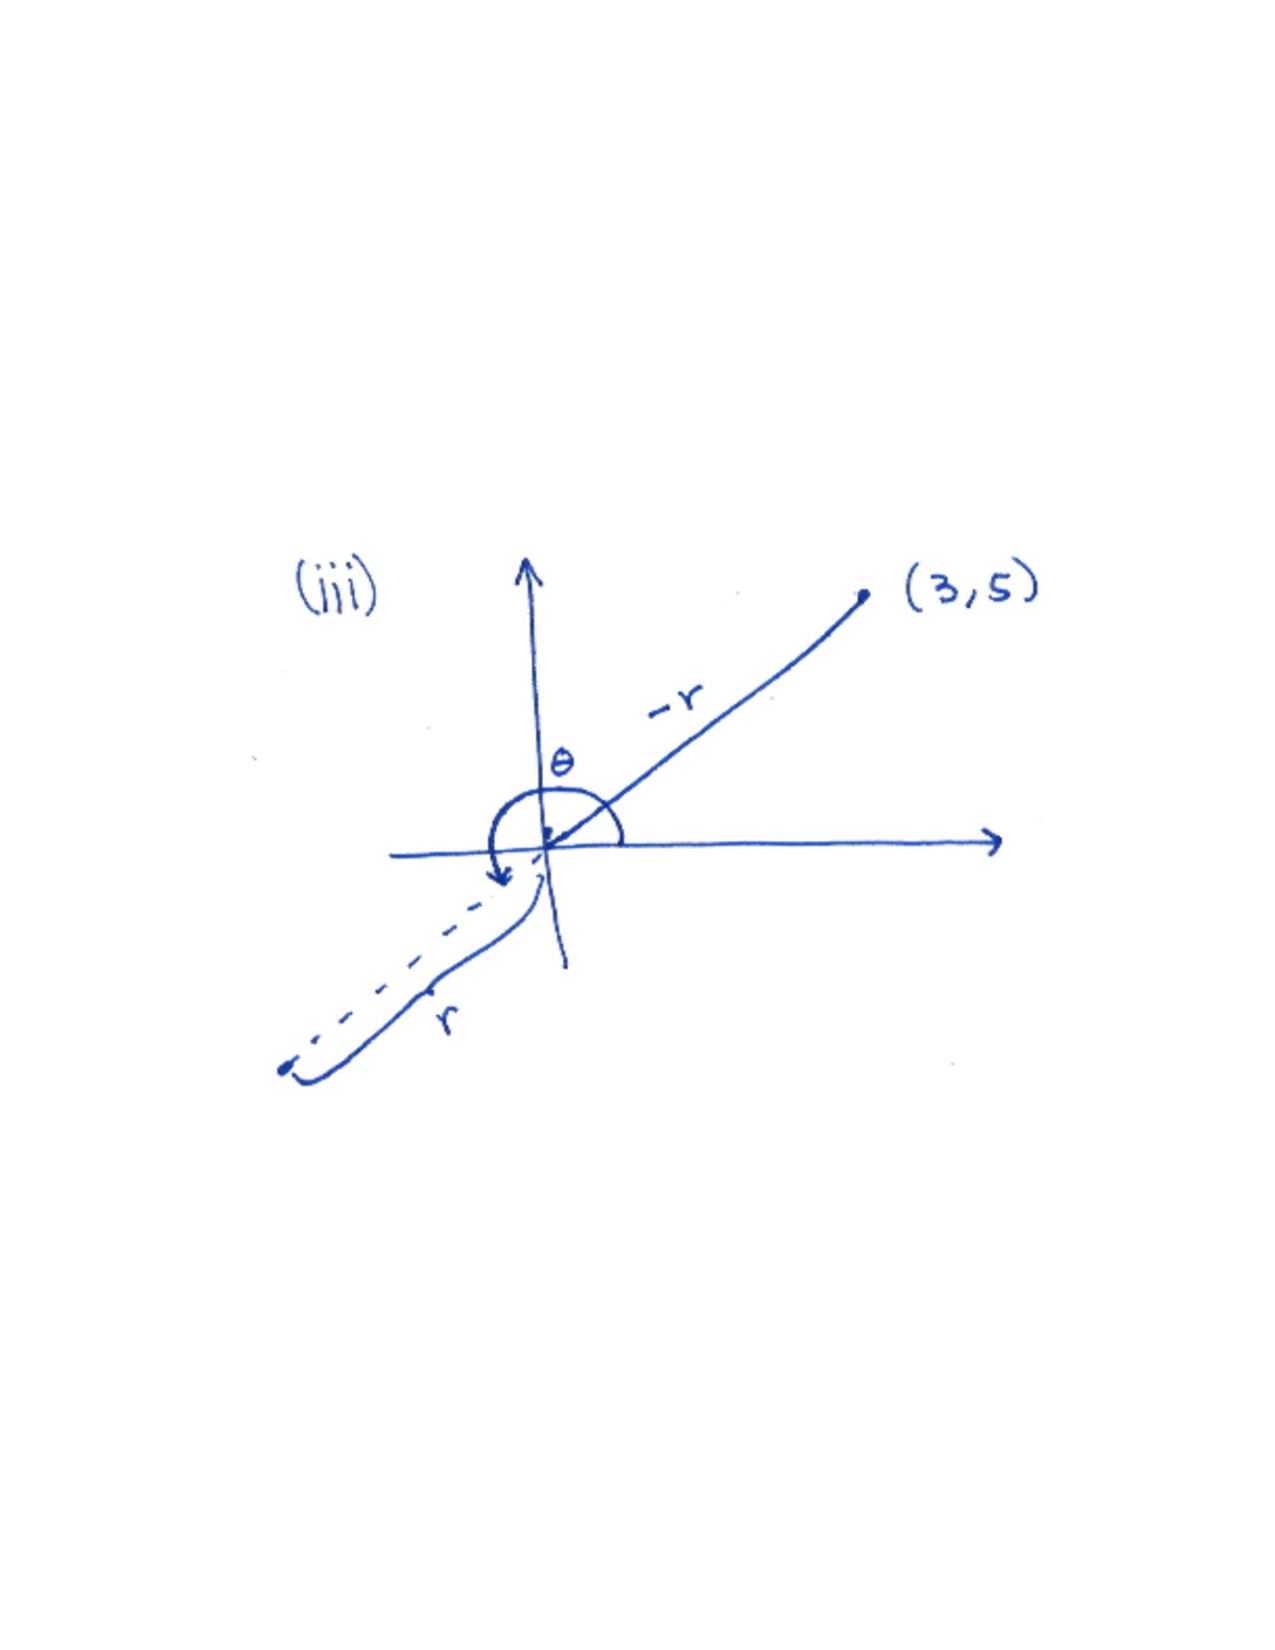
\includegraphics[trim= 170 290 170 260, scale=0.6]{Figure11-2-8.pdf}
		\end{image}
	
	\end{enumerate}
	\end{freeResponse}
		
\end{problem}

\begin{instructorNotes}
See problem 5.
\end{instructorNotes}







%problem 3
\begin{problem}
The graph of the curve $r = 4 \sin \theta$ is a circle. Use the graph below to sketch this circle. 
Can you verify this algebraically?  
What is the period of the polar curve?  
Is $0 \leq \theta \leq 2 \pi$ necessary to complete the graph?
	
	\begin{image}
	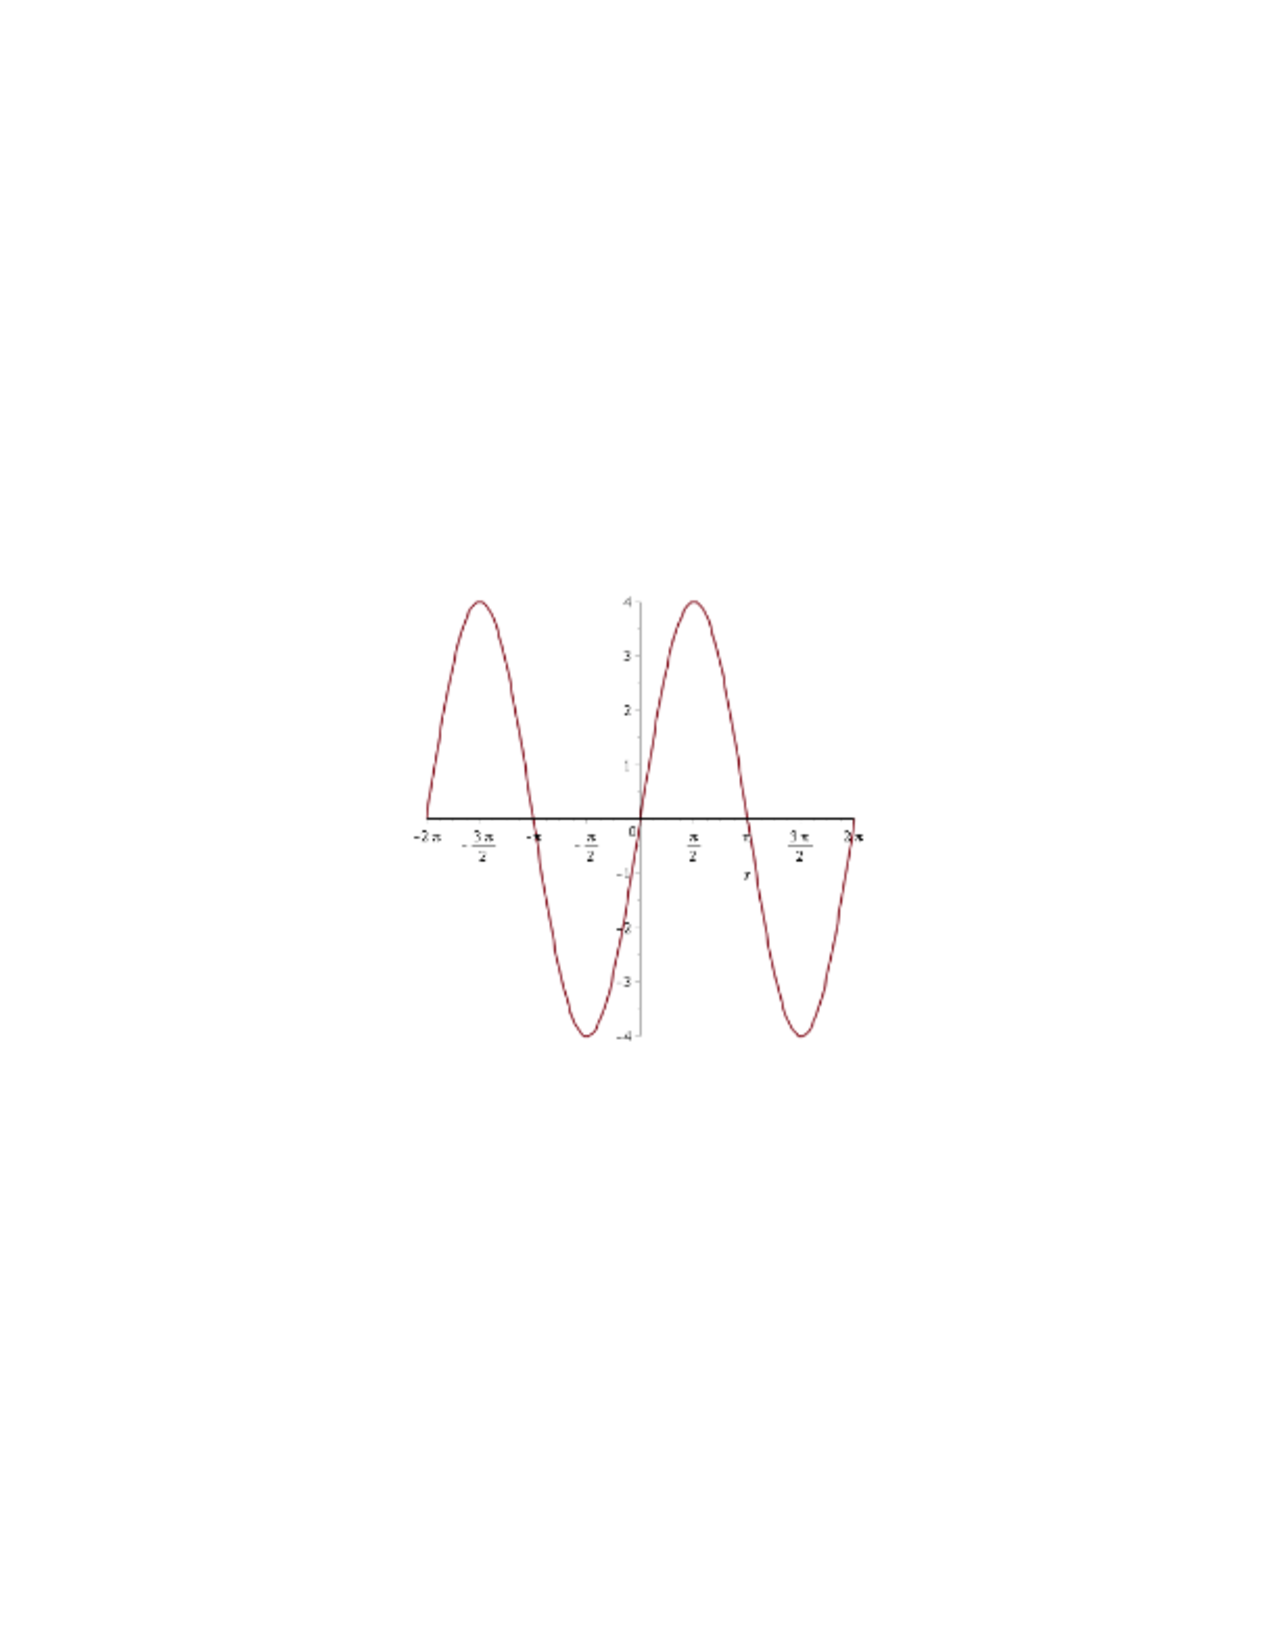
\includegraphics[trim= 170 290 170 280, scale=1]{Figure11-2-1.pdf}
	\end{image}

	\begin{freeResponse}
	Graphing this equation in the picture below, we see that this is a circle with radius $2$ and center $(0,2)$.  
	
	\begin{image}
	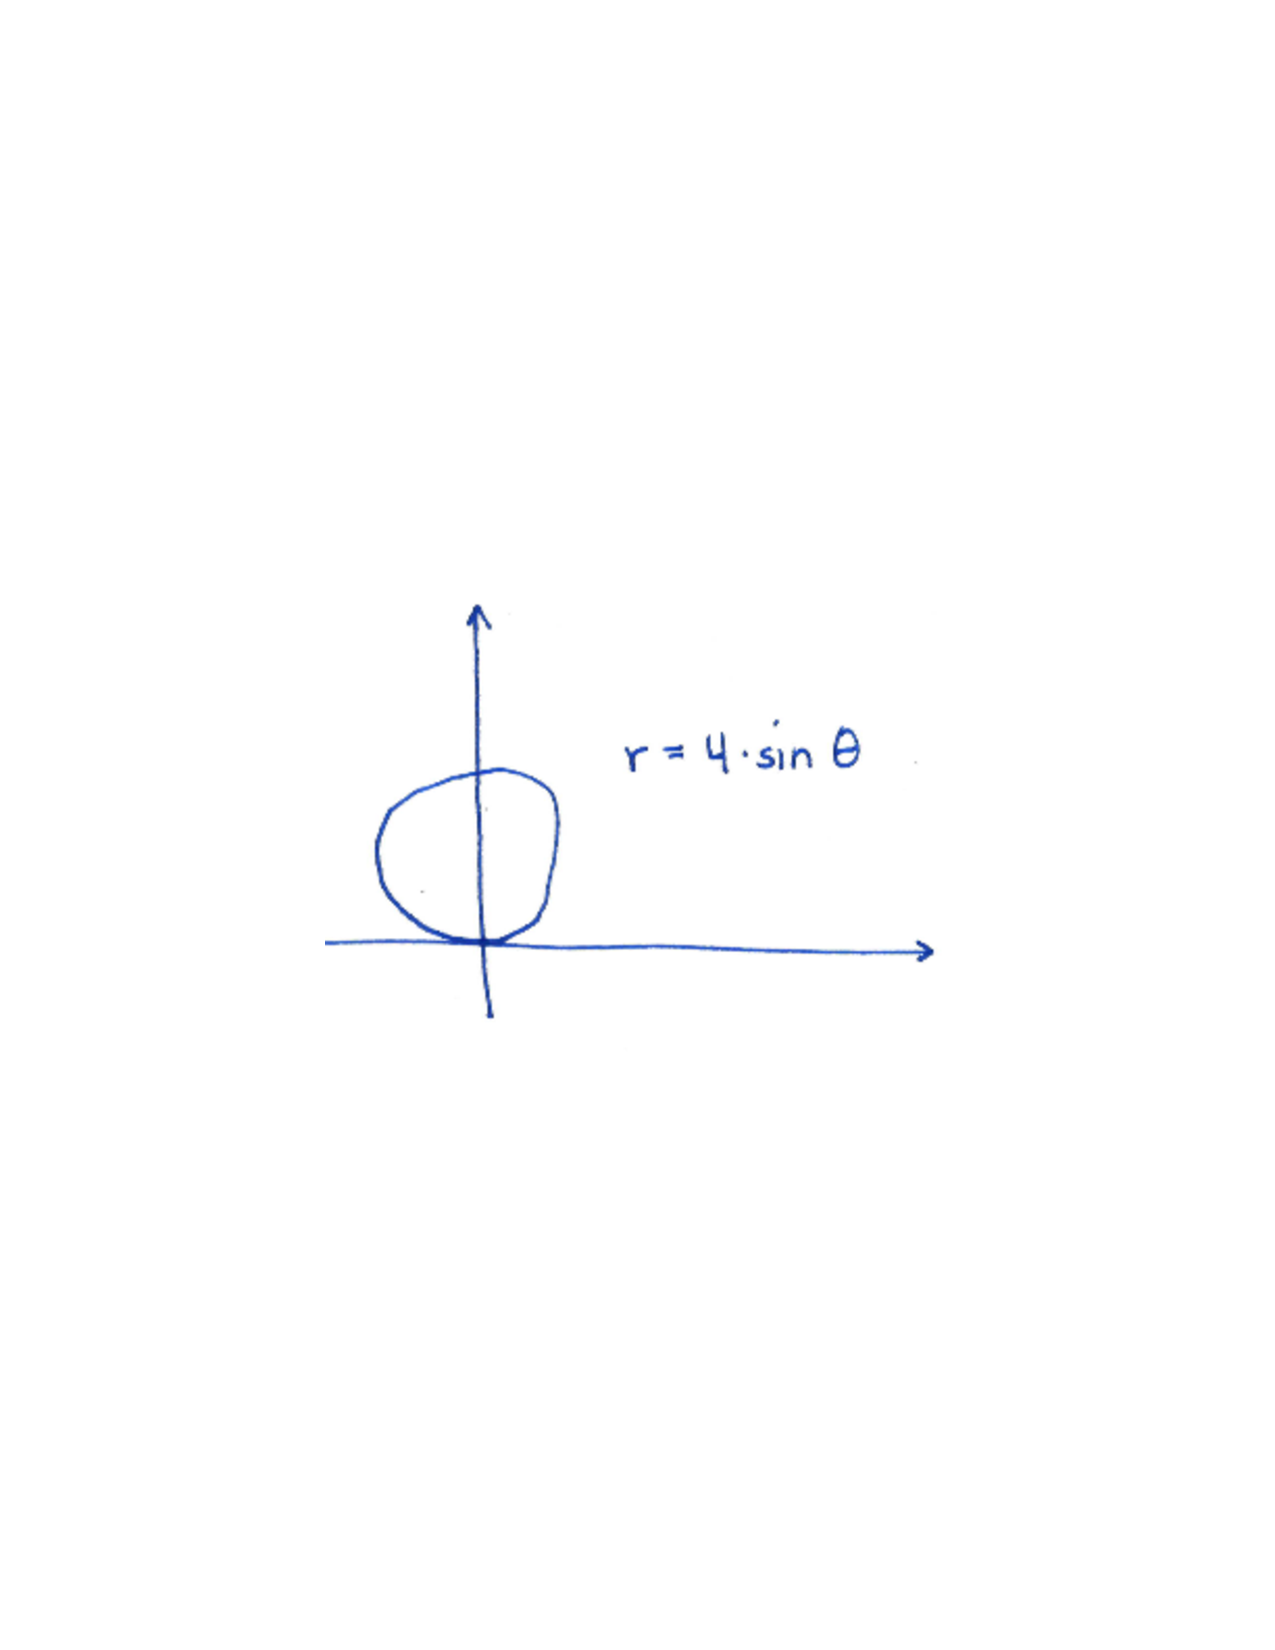
\includegraphics[trim= 170 310 170 290, scale=0.8]{Figure11-2-9.pdf}
	\end{image}
	
	To verify this algebraically,
		\begin{align*}
		4 = 4 \sin \theta \qquad
		&\Longrightarrow 	\qquad	r^2 = 4r \sin \theta  \\
		&\Longrightarrow 	\qquad	x^2 + y^2 = 4y  \\
		&\Longrightarrow 	\qquad	x^2 + y^2 - 4y = 0  \\
		&\Longrightarrow 	\qquad	x^2 + y^2 - 4y + 4 = 4  \\
		&\Longrightarrow 	\qquad	x^2 + (y-2)^2 = 2^2.
		\end{align*}
		
	To find the period of the polar curve, we convert both $x$ and $y$ into parametric equations with parameter $\theta$.  
		\begin{align*}
		&x = r \cos \theta = 4 \sin \theta \cos \theta = 2 \sin (2 \theta)  \\
		&y = r \sin \theta = 4 \sin^2 \theta = 4 \cdot \frac{1}{2} (1 - \cos(2 \theta)) = 2(1 - \cos(2 \theta)).
		\end{align*}
	The period of both $\sin(2 \theta)$ and $\cos(2 \theta)$ is $\pi$.  
	So the entire graph of the equation $r = 4 \sin \theta$ is traversed over the region $0 \leq \theta < \pi$.
	\end{freeResponse}

\end{problem}

\begin{instructorNotes}
Students sometimes have difficulty with the ``Cartesian to Polar'' graphing method given in the textbook.  
This will be important in the next section when they need to visualize curves in order to integrate in polar coordinates.
\end{instructorNotes}







%problem 4
\begin{problem}
Graph $r = 2 + 4 \cos \theta$ using the ``Cartesian-to-Polar'' method.
	\begin{freeResponse}
	First, we graph $r = 2 + 4 \cos \theta$ as if $r$ and $\theta$ were Cartesian coordinates.
	
	\begin{image}
	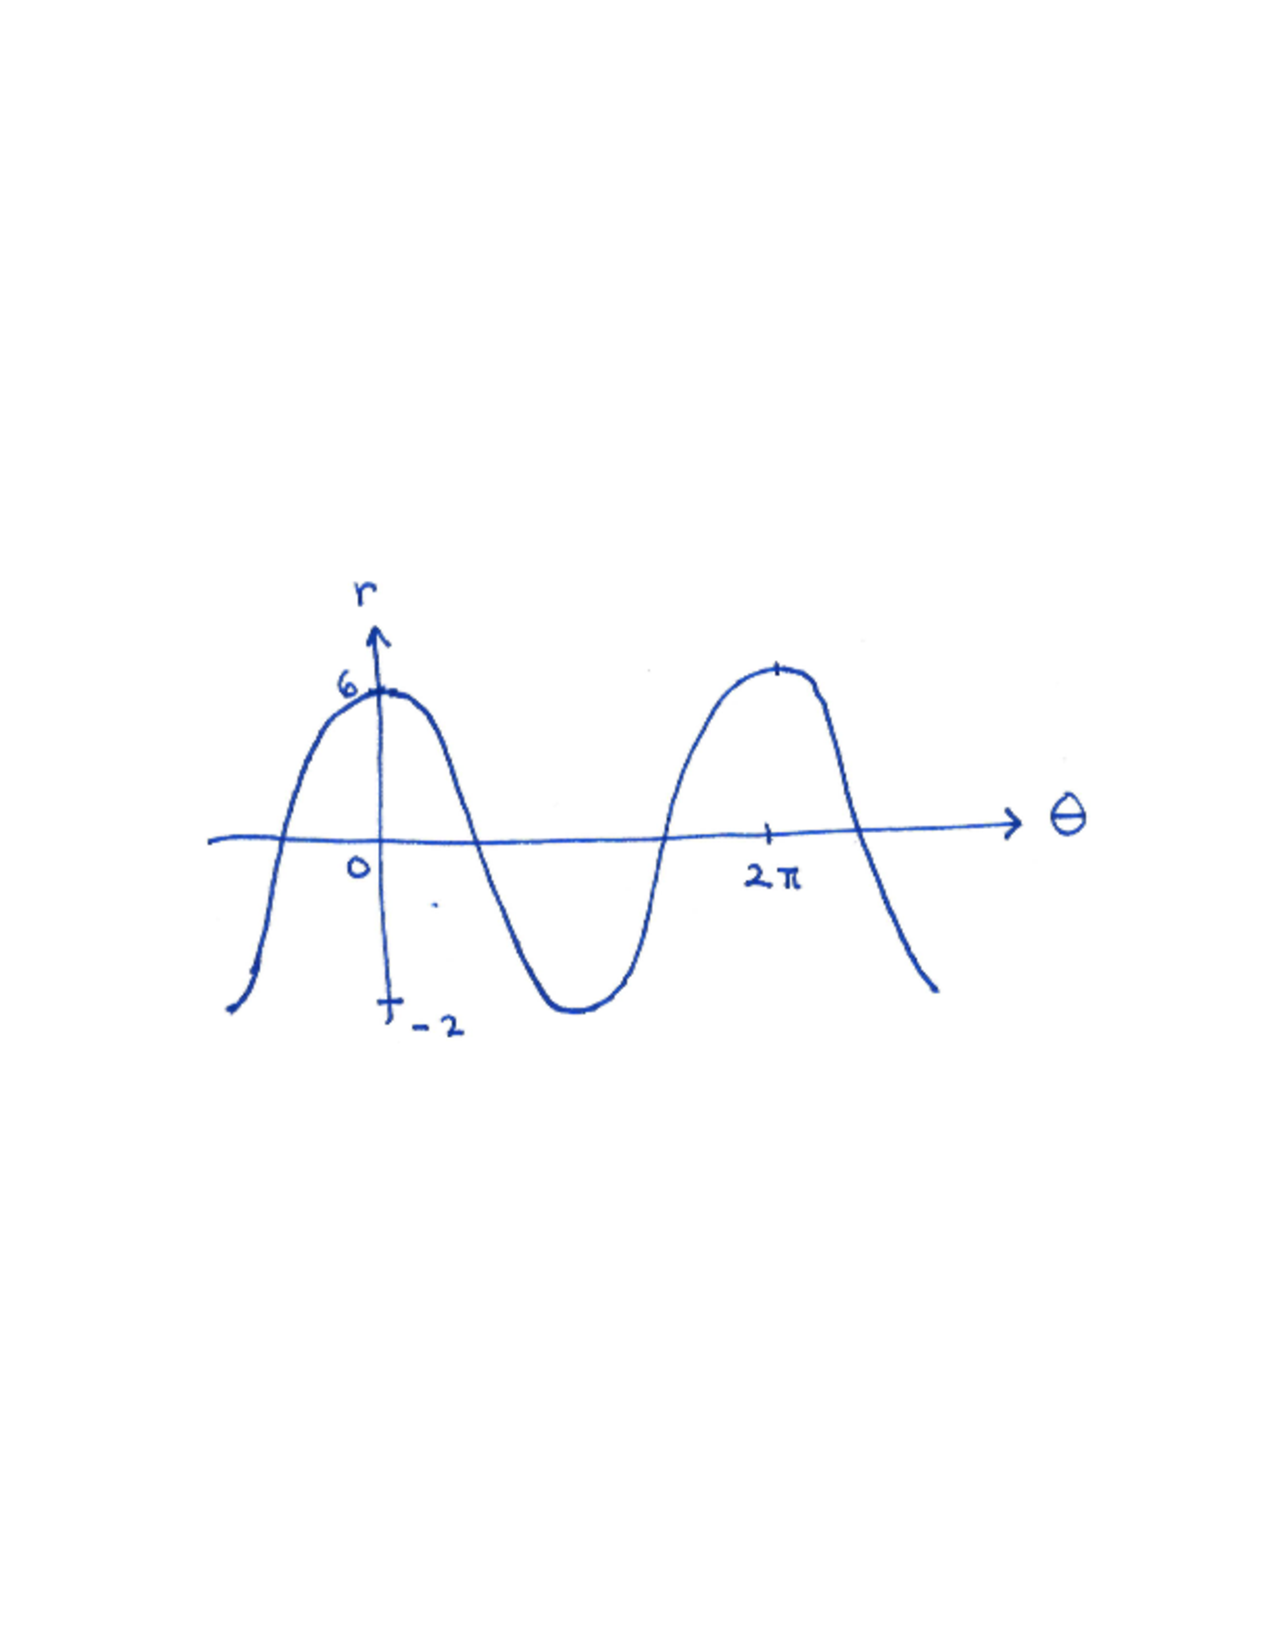
\includegraphics[trim= 170 310 170 290, scale=0.8]{Figure11-2-10.pdf}
	\end{image}
	
	We then use this to draw the following graph in the $xy$-plane
	
	\begin{image}
	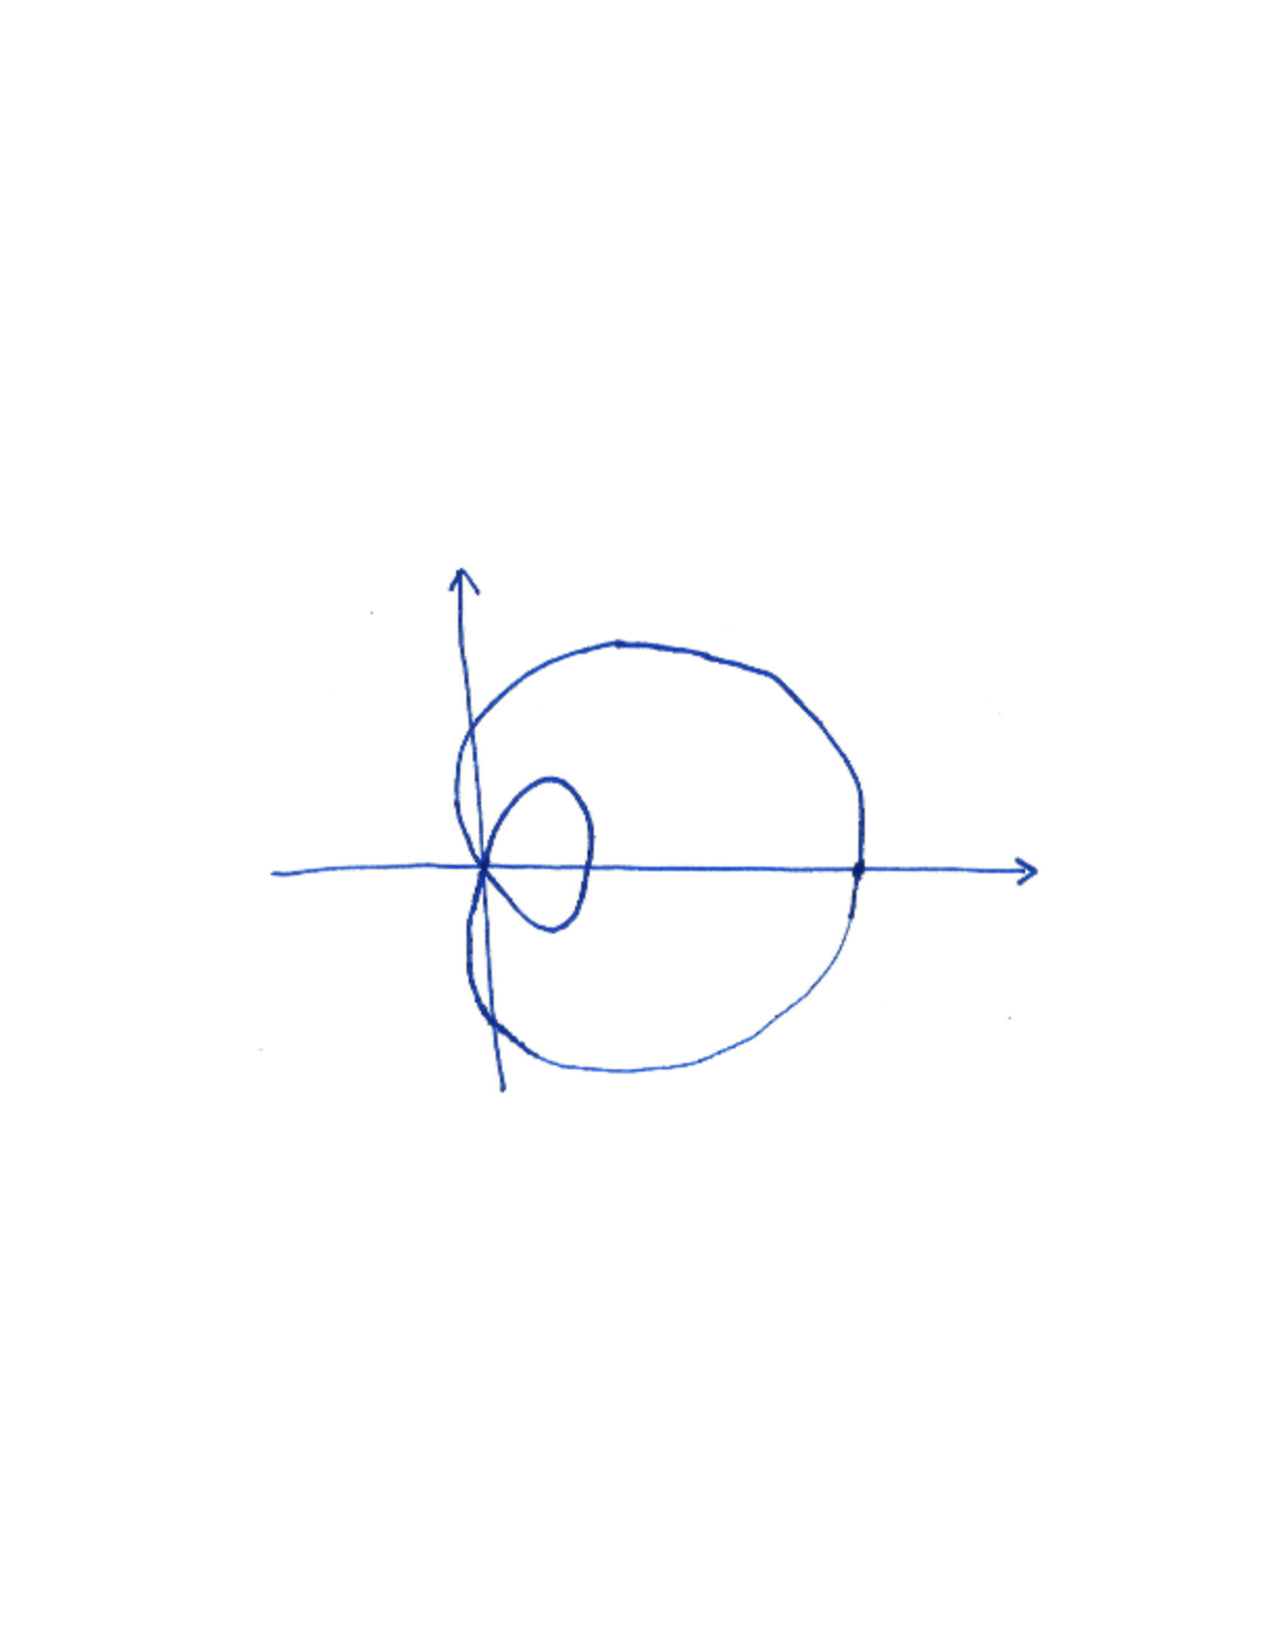
\includegraphics[trim= 170 270 170 270, scale=0.7]{Figure11-2-11.pdf}
	\end{image}
	
	If it helps, here are the parametric equations for this graph
		\begin{align*}
		&x = r \cos \theta = (2 + 4 \cos \theta) \cos \theta = 2 \cos \theta + 4 \cos^2 \theta = 2(\cos \theta + 1 + \cos(2 \theta)) \\
		&y = 4 \sin \theta = (2 + 4 \cos \theta) \sin \theta = 2 \sin \theta + 2 \sin (2 \theta).
		\end{align*}
	
	\end{freeResponse}

\end{problem}

\begin{instructorNotes}
See problem 7.
\end{instructorNotes}








\end{document} 




